\documentclass{article}

\usepackage{fullpage}
\usepackage[colorlinks=true]{hyperref}
\usepackage[tableposition=top]{caption}
\usepackage[utf8]{inputenc}

\usepackage{Sweave}
\begin{document}
\Sconcordance{concordance:MaternalParticulateMitoBiogen.tex:MaternalParticulateMitoBiogen.Rnw:%
1 7 1 1 0 7 1 1 19 1 1 1 48 1 43 1 1 1 14 1 2 6 1 1 14 1 2 6 1 1 14 1 2 %
6 1 1 14 1 2 6 1 1 14 1 2 6 1 1 14 1 2 6 1 1 53 1 2 4 1 2 2 11 0 1 2}


\title{Analysis of mitochondrial biogenesis genes in quadriceps muscle from the pups of the maternal particulate inhalation study}
\author{Erin Stephenson}
\date{\today}
\maketitle

This script uses the \verb+Sheet1+ from \verb+MaternalParticulatemtMitoBiogen.xlsx+ and is located in the \verb+C:/Users/esteph16/Documents/GitHub/ObesityParticulateTreatment/scripts/MitoBiogenGenes+ directory.  This analysis was most recently run on Tue Feb 09 16:58:48 2016.  

\section*{Statistics}
\begin{figure}
\begin{center}
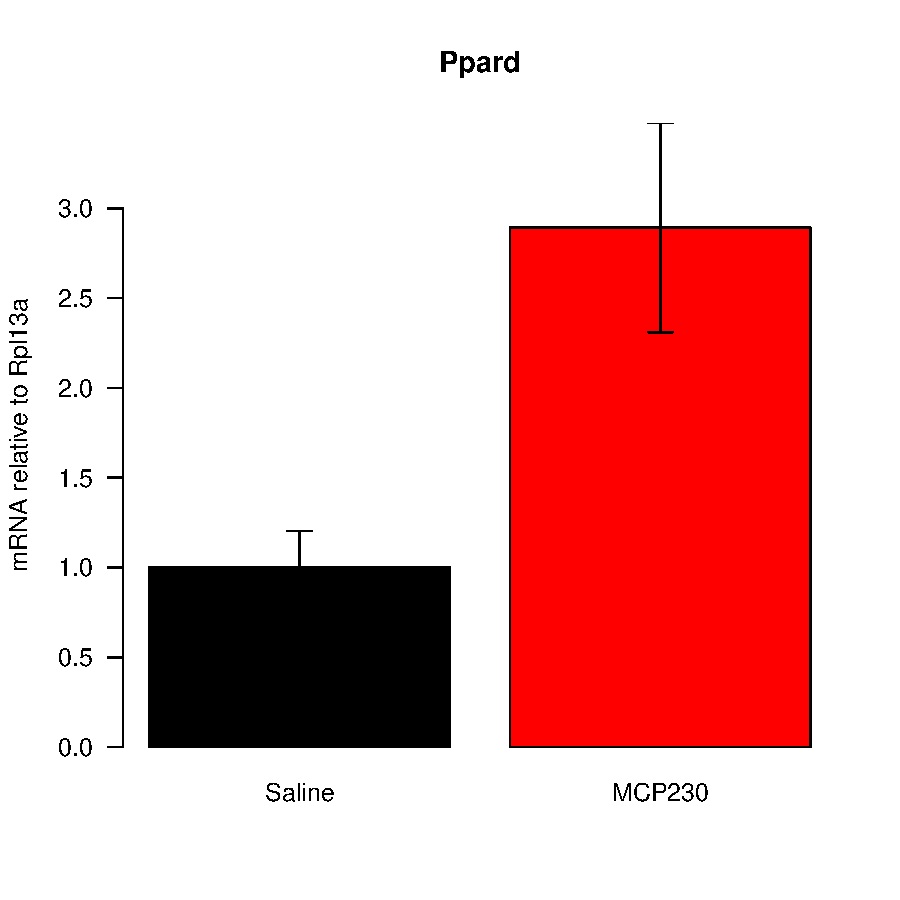
\includegraphics{MaternalParticulateMitoBiogen-barplotPpard}
\end{center}
\caption{Barplot of Ppard mRNA}
\label{fig:barplotPpard}
\end{figure}

\begin{figure}
\begin{center}
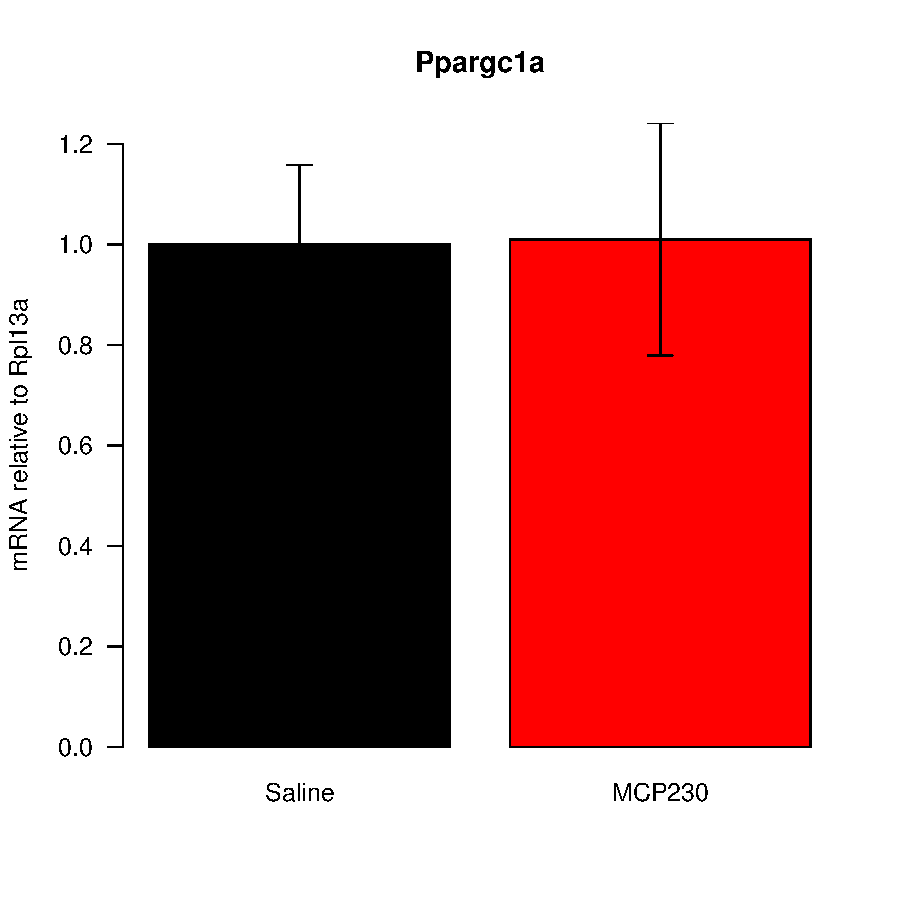
\includegraphics{MaternalParticulateMitoBiogen-barplotPpargc1a}
\end{center}
\caption{Barplot of Ppargc1a mRNA}
\label{fig:barplotPpargc1a}
\end{figure}

\begin{figure}
\begin{center}
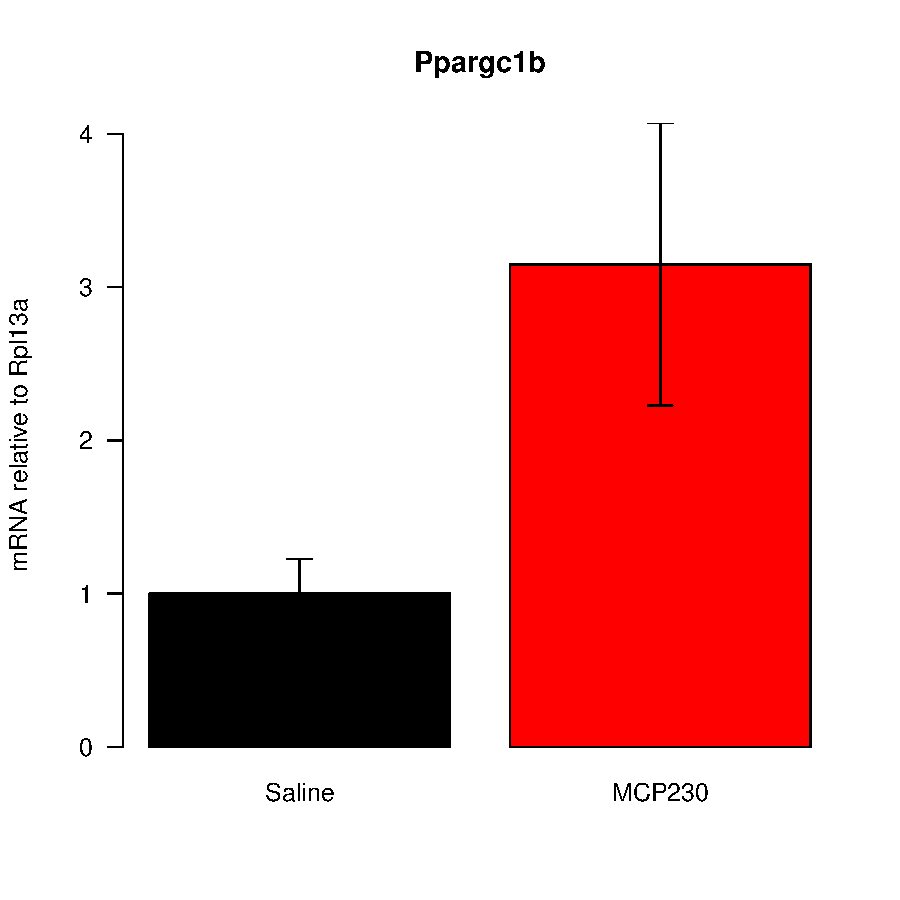
\includegraphics{MaternalParticulateMitoBiogen-barplotPpargc1b}
\end{center}
\caption{Barplot of Ppargc1b mRNA}
\label{fig:barplotPpargc1b}
\end{figure}

\begin{figure}
\begin{center}
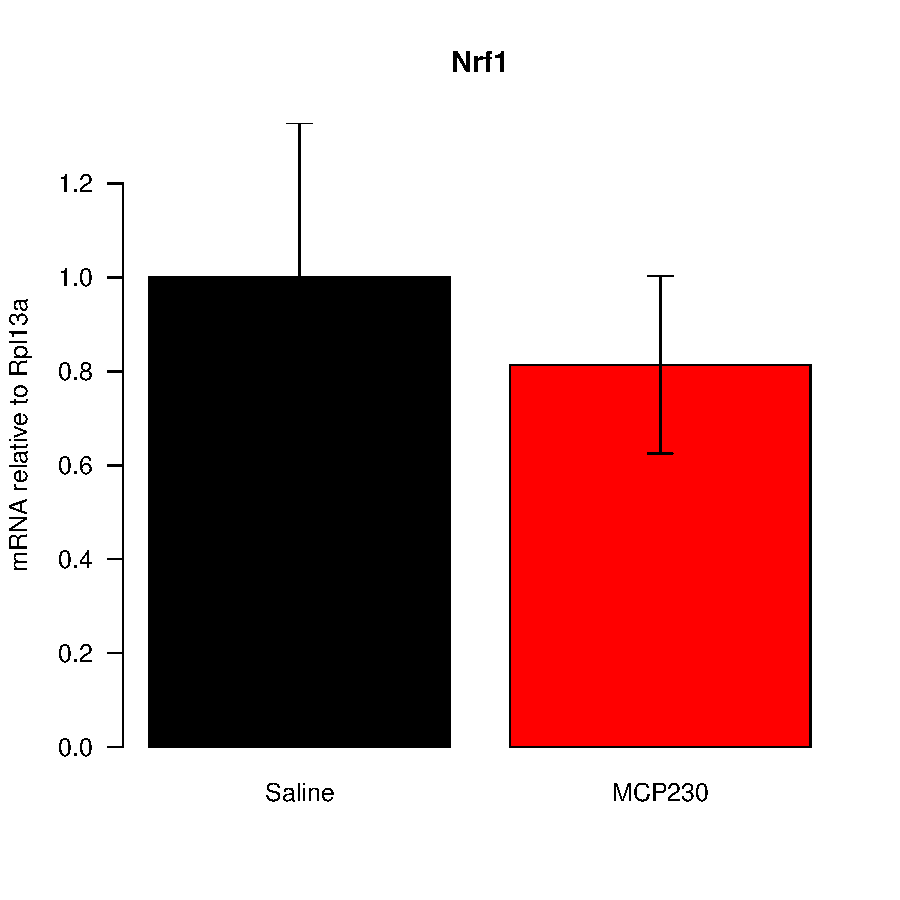
\includegraphics{MaternalParticulateMitoBiogen-barplotNrf1}
\end{center}
\caption{Barplot of Nrf1 mRNA}
\label{fig:barplotNrf1}
\end{figure}

\begin{figure}
\begin{center}
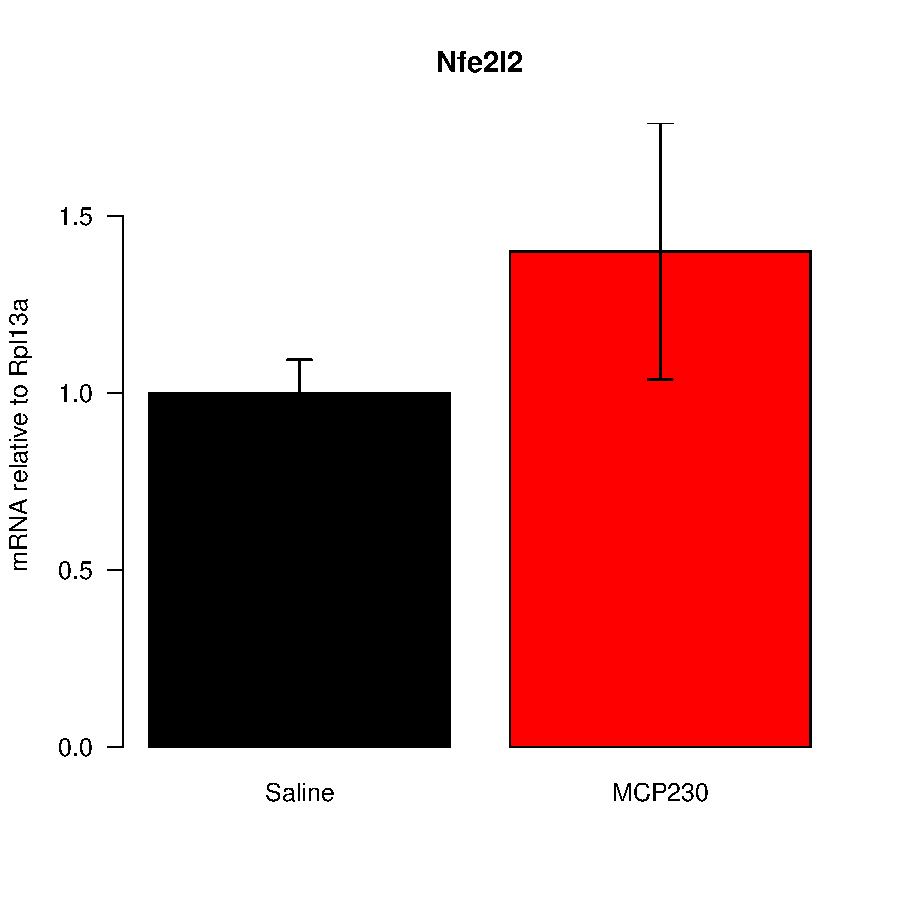
\includegraphics{MaternalParticulateMitoBiogen-barplotNfe2l2}
\end{center}
\caption{Barplot of Nfe2l2 mRNA}
\label{fig:barplotNfe2l2}
\end{figure}

\begin{figure}
\begin{center}
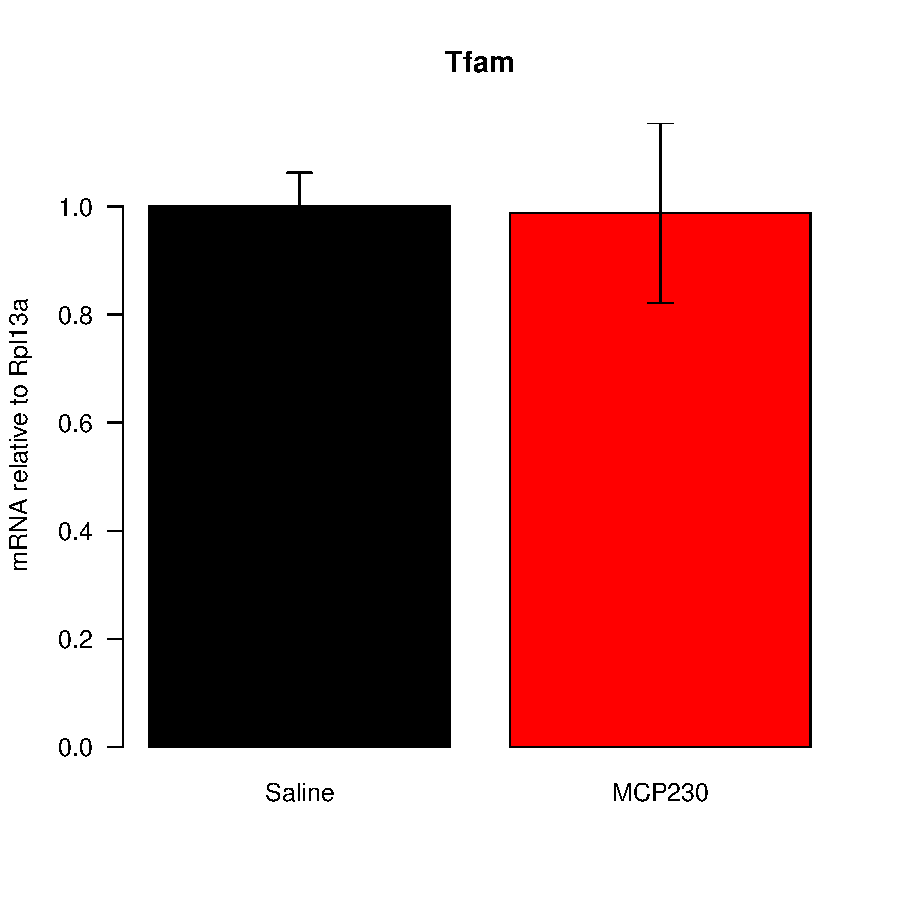
\includegraphics{MaternalParticulateMitoBiogen-barplotTfam}
\end{center}
\caption{Barplot of Tfam mRNA}
\label{fig:barplotTfam}
\end{figure}

\begin{figure}
\begin{center}
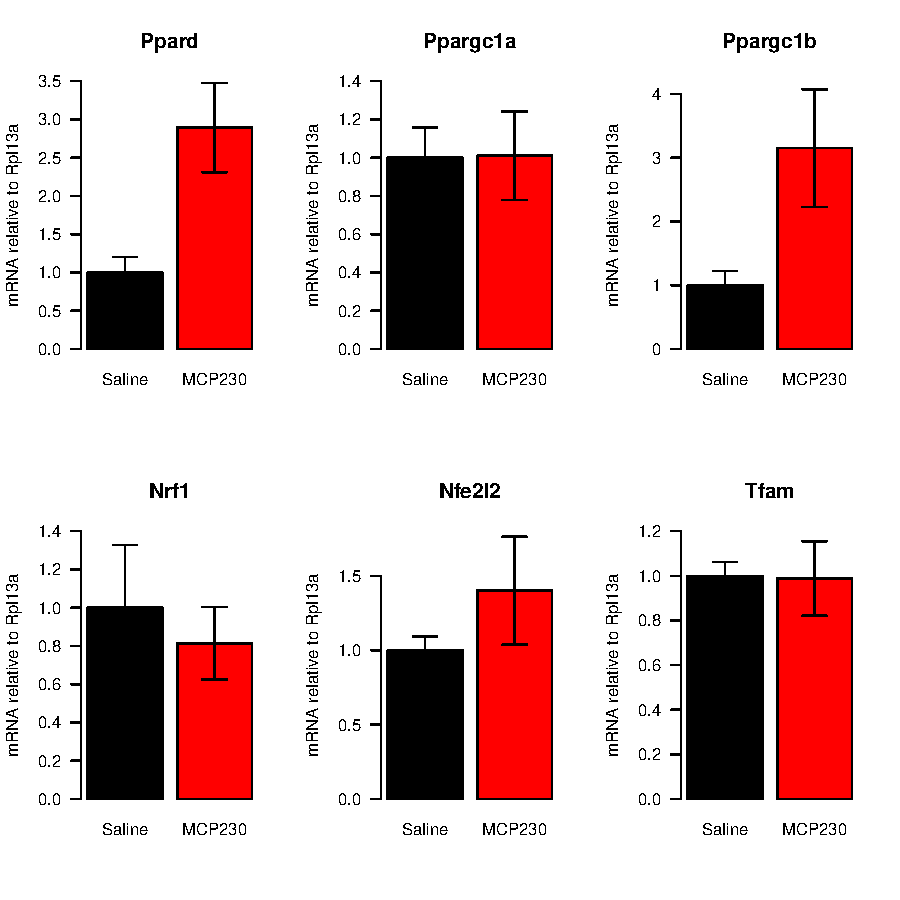
\includegraphics{MaternalParticulateMitoBiogen-barplot-combined}
\end{center}
\caption{Barplot of the mitochondrial biogenesis genes}
\label{fig:barplot-combined}
\end{figure}

\section*{Session Information}
\begin{itemize}\raggedright
  \item R version 3.1.1 (2014-07-10), \verb|x86_64-w64-mingw32|
  \item Locale: \verb|LC_COLLATE=English_United States.1252|, \verb|LC_CTYPE=English_United States.1252|, \verb|LC_MONETARY=English_United States.1252|, \verb|LC_NUMERIC=C|, \verb|LC_TIME=English_United States.1252|
  \item Base packages: base, datasets, graphics, grDevices, methods,
    stats, utils
  \item Other packages: car~2.0-25, plyr~1.8.3, rJava~0.9-7,
    xlsx~0.5.7, xlsxjars~0.6.1
  \item Loaded via a namespace (and not attached): grid~3.1.1,
    lattice~0.20-29, lme4~1.1-10, MASS~7.3-33, Matrix~1.2-3,
    MatrixModels~0.4-1, mgcv~1.8-0, minqa~1.2.4, nlme~3.1-117,
    nloptr~1.0.4, nnet~7.3-8, parallel~3.1.1, pbkrtest~0.4-4,
    quantreg~5.19, Rcpp~0.12.2, SparseM~1.7, splines~3.1.1, tools~3.1.1
\end{itemize}\end{document}
